\documentclass[11pt,a4paper]{article}

% ---------------------------------------------------------------------------
% MedSkel AI -- project report (Neural Networks and Deep Learning course)
% Build: latexmk -pdf report_medskel_ai_en.tex
% Figures in figures/private/ contain FIVES images (CC BY 4.0): they are not
% committed to Git (repository rule) but are needed to compile.
% ---------------------------------------------------------------------------

\usepackage[T1]{fontenc}
\usepackage[utf8]{inputenc}
\usepackage[english]{babel}
\usepackage{lmodern}
\usepackage{microtype}
\usepackage[margin=2.4cm]{geometry}
\usepackage{amsmath,amssymb,bm,mathtools}
\usepackage{booktabs,tabularx,multirow}
\usepackage{graphicx}
\usepackage{caption}
\usepackage{xcolor}
\usepackage{tikz}
\usetikzlibrary{arrows.meta,positioning,calc}
\usepackage{enumitem}
\usepackage{fancyhdr}
\usepackage{titlesec}
\usepackage[hidelinks]{hyperref}

\definecolor{teal}{HTML}{0F8B8D}
\definecolor{ink}{HTML}{1E2A33}
\definecolor{soft}{HTML}{EEF6F6}
\definecolor{warn}{HTML}{B5532A}

\titleformat{\section}{\Large\bfseries\color{teal}}{\thesection}{0.6em}{}
\titleformat{\subsection}{\large\bfseries\color{ink}}{\thesubsection}{0.6em}{}
\captionsetup{font=small,labelfont=bf}
\setlist{itemsep=1pt,topsep=3pt}
\pagestyle{fancy}
\fancyhf{}
\fancyhead[L]{\small\color{teal}MedSkel AI}
\fancyhead[R]{\small Project report -- Neural Networks and Deep Learning}
\fancyfoot[C]{\small\thepage}
\renewcommand{\headrulewidth}{0.3pt}
\newcommand{\pct}{\%}

\begin{document}

% ---------------------------------------------------------------------------
\begin{titlepage}
\centering
{\large School of Digital Engineering and Artificial Intelligence (EIDIA)\par}
{\large Euromed University of Fes\par}
\vspace{2.6cm}
{\Huge\bfseries\color{teal} MedSkel AI\par}
\vspace{0.5cm}
{\LARGE Retinal vessel segmentation with a U-Net\\[2pt] and geometric measurement of the vessels\par}
\vspace{1.4cm}
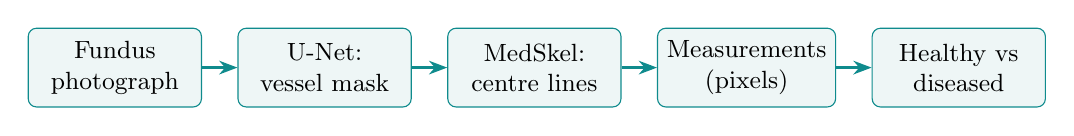
\begin{tikzpicture}[node distance=0.45cm, every node/.style={font=\small}]
  \tikzstyle{stp}=[rectangle,rounded corners=3pt,draw=teal,fill=soft,minimum width=2.2cm,minimum height=1.0cm,align=center]
  \node[stp] (a) {Fundus\\photograph};
  \node[stp,right=of a] (b) {U-Net:\\vessel mask};
  \node[stp,right=of b] (c) {MedSkel:\\centre lines};
  \node[stp,right=of c] (d) {Measurements\\(pixels)};
  \node[stp,right=of d] (e) {Healthy vs\\diseased};
  \foreach \x/\y in {a/b,b/c,c/d,d/e} \draw[-{Stealth},thick,teal] (\x) -- (\y);
\end{tikzpicture}
\vspace{2cm}

{\large Project report\par}
{Course: Neural Networks and Deep Learning\par}
{Instructor: Prof. N. Joudar\par}
\vfill
{\Large Mouhssine El Boumshouli\par}
{4th year, engineering cycle\par}
\vspace{0.4cm}
{November 2026\par}
{\small Code: \url{https://github.com/MouhssineElBoumshouli/medskel-ai}\par}
\end{titlepage}

% ---------------------------------------------------------------------------
\section*{Abstract}
We train a U-Net in PyTorch, with no pre-trained weights (7{,}849{,}601 parameters), to mark the blood vessels in photographs of the back of the eye (fundus photographs). The data come from the public FIVES dataset (800 expert-annotated images of $2048\times2048$ pixels, four groups: healthy, age-related macular degeneration (AMD), diabetic retinopathy, glaucoma). Training runs on a 4\,GB laptop GPU, on $512\times512$ pixel tiles. Every decision is made on a separate validation set; the official test set is used only at the end.

The final model reaches a \textbf{mean Dice of 0.889} (95\pct\ interval: 0.873 -- 0.903) on the 200 FIVES test images. A U-Net with a pre-trained ResNet34 encoder, used as a reference, reaches 0.907. On an external dataset from another camera (CHASE\_DB1, 28 images of 14 children), our model reaches a Dice of 0.766 against the first expert, versus 0.777 for the second human expert; it does, however, mark more pixels than the experts. The main weakness is the thinnest vessels (recall of 0.46).

We then connect the network to the geometric method MedSkel (centre lines from bisectors, Saidou et al., 2024) to measure the vessels. With MedSkel, the number of branch points changes half as much as with classical thinning when the expert mask is replaced by the network mask (26\pct\ vs 53\pct). Eyes with AMD, diabetic retinopathy or glaucoma show lower vessel density, fractal dimension, total length and number of branch points than healthy eyes ($p<0.001$). These measurements are, however, not enough to classify a single eye (balanced accuracy 0.45 to 0.49 for 4 groups). This is a research tool, not a diagnostic device.

\tableofcontents
\newpage

% ---------------------------------------------------------------------------
\section{Introduction}

\subsection{Context}
The retina is the only place in the body where blood vessels can be seen without surgery, with a simple photograph of the back of the eye. The shape of these vessels (density, width, branching, tortuosity) is studied in research because it is associated with eye and general diseases: diabetic retinopathy, glaucoma, hypertension. A recent study of 10{,}151 healthy UK Biobank participants linked 114 vessel features to age, blood pressure, BMI and HbA1c \cite{yusufu}.

Before measuring, the vessels must be \textbf{found}, pixel by pixel. This is a \textbf{semantic segmentation} problem: for each pixel, decide whether it belongs to a vessel. Manual tracing by an expert is slow, and two experts do not trace exactly the same thing.

\subsection{Starting point}
An earlier project, \texttt{medskel}, implements a geometric centre-line method inspired by Saidou et al.\ \cite{saidou}. Its weak point was the first step: vessels were detected with a classical filter (Frangi filter), which is unreliable. This project replaces that filter with a convolutional neural network, then reuses MedSkel to measure.

\subsection{Goals and contributions}
\begin{enumerate}
  \item Build and explain a complete U-Net in PyTorch, trained from scratch on real annotations (FIVES).
  \item Evaluate it honestly: strict train / validation / test separation, confidence intervals, an external test on another dataset, and a comparison with a second human expert.
  \item Find the main weakness (thin vessels) and test improvements one at a time.
  \item Connect the network mask to MedSkel to obtain measurements, and check their stability and their link with the disease groups.
  \item Deliver a local application that runs all the steps.
\end{enumerate}

% ---------------------------------------------------------------------------
\section{Data}

\subsection{FIVES}
FIVES \cite{fives} contains 800 colour fundus photographs (TRC-NW8 camera, 50° field, $2048\times2048$ pixels) of 573 patients, each with a binary vessel mask drawn by experts. The images form four groups of 200: AMD (A), diabetic retinopathy (D), glaucoma (G) and healthy (N). The authors define 600 training and 200 test images.

We first audited the data (script \texttt{python -m medskel\_ai.data}):
\begin{itemize}
  \item 800 image/mask pairs with the same name and size; masks strictly binary (0 and 255);
  \item vessels cover on average 7.5\pct\ of pixels (N: 9.0\pct; A: 7.3\pct; D: 6.9\pct; G: 6.7\pct);
  \item \textbf{2 completely black masks} in training (447\_G, 448\_G): annotation errors, excluded;
  \item \textbf{6 pairs of byte-identical photographs} (5 in training, 1 in test, none across the two): each pair is kept on the same side of the split.
\end{itemize}

\textbf{Split.} Of the 598 usable training images, 88 form the validation set (22 per group, seed 42) and 510 are used for training. The same split is used in every experiment.

\begin{center}
\begin{tabular}{@{}lcl@{}}
\toprule
\textbf{Set} & \textbf{Images} & \textbf{Role} \\
\midrule
Training & 510 & learning the weights \\
Validation & 88 & every decision (threshold, stopping, choice of experiments) \\
Test (official) & 200 & final score only \\
\bottomrule
\end{tabular}
\end{center}

\subsection{CHASE\_DB1 (external test)}
CHASE\_DB1 \cite{chase} contains 28 photographs (both eyes of 14 children), taken with another camera (Nidek NM-200-D, 30°, $999\times960$ pixels). Each image has \textbf{two} masks drawn independently by two observers, which lets us measure the agreement between two humans. No CHASE image was used to train, to choose a model or to set a threshold.

\subsection{Limitation}
The 800 FIVES images come from 573 patients and no patient identifier is published: two photographs of the same patient may sit on both sides of the split. The scores are therefore on \emph{images} never seen, not on \emph{patients} proven never seen.

% ---------------------------------------------------------------------------
\section{Method: the U-Net}

\subsection{Convolution}
A convolution layer slides a small learned filter over the image. For an input $X$ with $C$ channels and a $3\times3$ filter $W$, the output at pixel $(i,j)$ is
\begin{equation}
Y(i,j) \;=\; b \;+\; \sum_{c=1}^{C}\sum_{u=-1}^{1}\sum_{v=-1}^{1} W(c,u,v)\; X(c,\,i+u,\,j+v).
\end{equation}
Example: the filter $\begin{psmallmatrix}-1&2&-1\\-1&2&-1\\-1&2&-1\end{psmallmatrix}$ responds $3\times(2\times9)=54$ on a vertical line of value 9, and $0$ on a horizontal line or a flat area: it is a vertical-line detector. The weights $W$ and the bias $b$ are not chosen by hand: they are \textbf{learned}. Each layer uses several filters, each producing a \emph{feature map}. Zero padding keeps the image size.

\subsection{Non-linearity, normalisation and downsampling}
\begin{itemize}
  \item \textbf{ReLU}: $\mathrm{ReLU}(x)=\max(0,x)$. Without it, a stack of convolutions would collapse into a single linear operation.
  \item \textbf{Batch normalisation} \cite{bn}: each channel is re-centred and re-scaled,
  $\hat{x} = \gamma\,\frac{x-\mu_B}{\sqrt{\sigma_B^2+\varepsilon}} + \beta$, which stabilises and speeds up learning.
  \item \textbf{$2\times2$ max pooling}: keep the maximum of each $2\times2$ block. The map becomes half as large; the next filters see a larger area of the image (the context needed to tell a vessel from a dark spot), at the cost of exact position.
\end{itemize}

\subsection{Architecture}
The U-Net \cite{unet} is a symmetric encoder--decoder (figure~\ref{fig:unet}).
\begin{itemize}
  \item \textbf{Encoder}: 4 blocks of 32, 64, 128 and 256 channels. Each block = (3$\times$3 convolution, normalisation, ReLU) $\times 2$, then max pooling.
  \item \textbf{Bottleneck}: 512 channels, at $32\times32$ pixels for a $512\times512$ tile.
  \item \textbf{Decoder}: 4 steps of bilinear $\times2$ upsampling, then \textbf{concatenation} with the encoder map of the same size (\emph{skip connection}), then a convolution block.
  \item \textbf{Output}: a $1\times1$ convolution gives one \emph{logit} $z$ per pixel; the sigmoid $\sigma(z)=1/(1+e^{-z})$ turns it into a probability.
\end{itemize}
Skip connections are essential: the decoder knows \emph{what} is there (deep information), and the encoder maps bring back exactly \emph{where} (fine information). Without them, thin vessels disappear. The network has \textbf{7{,}849{,}601 parameters}, all learned from scratch.

\begin{figure}[h]
\centering
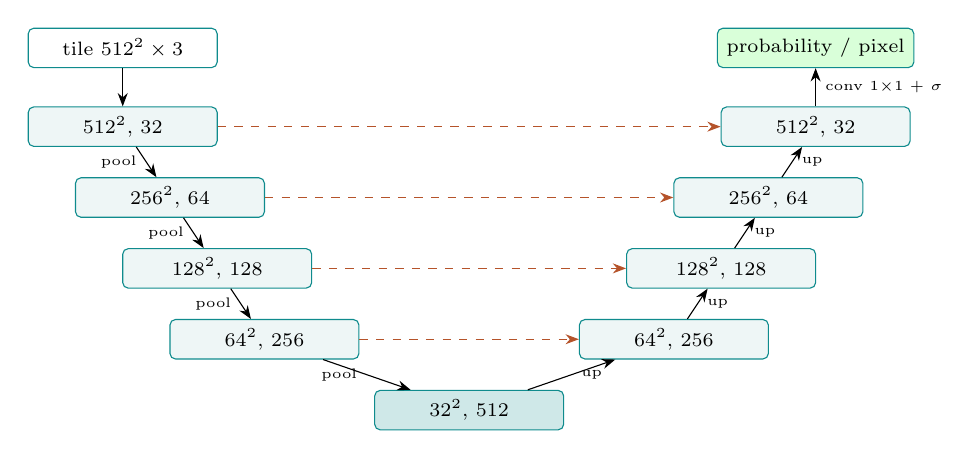
\begin{tikzpicture}[x=1cm,y=1cm,font=\scriptsize]
  \tikzstyle{blk}=[rectangle,draw=teal,fill=soft,minimum height=0.5cm,minimum width=2.4cm,align=center,rounded corners=2pt]
  \node[blk,fill=white] (in) at (0,1) {tile $512^2\times3$};
  \node[blk] (e1) at (0,0)    {$512^2$, 32};
  \node[blk] (e2) at (0.6,-0.9) {$256^2$, 64};
  \node[blk] (e3) at (1.2,-1.8) {$128^2$, 128};
  \node[blk] (e4) at (1.8,-2.7) {$64^2$, 256};
  \node[blk,fill=teal!20] (b) at (4.4,-3.6) {$32^2$, 512};
  \node[blk] (d4) at (7.0,-2.7) {$64^2$, 256};
  \node[blk] (d3) at (7.6,-1.8) {$128^2$, 128};
  \node[blk] (d2) at (8.2,-0.9) {$256^2$, 64};
  \node[blk] (d1) at (8.8,0)  {$512^2$, 32};
  \node[blk,fill=green!15] (out) at (8.8,1) {probability / pixel};
  \draw[-{Stealth}] (in) -- (e1);
  \foreach \a/\b in {e1/e2,e2/e3,e3/e4,e4/b} \draw[-{Stealth}] (\a) -- node[left]{\tiny pool} (\b);
  \foreach \a/\b in {b/d4,d4/d3,d3/d2,d2/d1} \draw[-{Stealth}] (\a) -- node[right]{\tiny up} (\b);
  \draw[-{Stealth}] (d1) -- node[right]{\tiny conv $1{\times}1$ + $\sigma$} (out);
  \foreach \a/\b in {e1/d1,e2/d2,e3/d3,e4/d4} \draw[-{Stealth},dashed,warn] (\a.east) -- (\b.west);
\end{tikzpicture}
\caption{The U-Net used here (spatial size, number of channels). Dashed arrows: skip connections (concatenation).}
\label{fig:unet}
\end{figure}

% ---------------------------------------------------------------------------
\section{Method: training}

\subsection{Loss function}
Let $y_k\in\{0,1\}$ be the ground truth and $p_k=\sigma(z_k)$ the predicted probability at pixel $k$, over $N$ pixels.

\textbf{Binary cross-entropy} (computed directly on the logits for numerical stability):
\begin{equation}
\mathcal{L}_{\text{BCE}} = -\frac{1}{N}\sum_{k}\Big[y_k\ln p_k + (1-y_k)\ln(1-p_k)\Big].
\end{equation}
For a vessel pixel, $p=0.9$ costs $-\ln 0.9\approx0.11$, while $p=0.1$ costs $-\ln0.1\approx2.30$: confident mistakes are punished hard.

\textbf{Soft Dice loss} \cite{vnet}:
\begin{equation}
\mathcal{L}_{\text{Dice}} = 1-\frac{2\sum_k p_k y_k + \epsilon}{\sum_k p_k + \sum_k y_k + \epsilon}.
\end{equation}
Because only 7.5\pct\ of pixels are vessels, BCE alone is dominated by the background. The Dice loss only looks at vessel overlap and balances this. We use $\mathcal{L}=\mathcal{L}_{\text{BCE}}+\mathcal{L}_{\text{Dice}}$ (equal weights).

\subsection{Backpropagation and optimisation}
Backpropagation computes the gradient $\nabla_\theta\mathcal{L}$ with respect to each of the 7.8 million parameters, applying the chain rule layer by layer, from the output back to the input. The parameters are updated with \textbf{Adam} \cite{adam}, with $g_t=\nabla_\theta\mathcal{L}$:
\begin{align}
m_t &= \beta_1 m_{t-1} + (1-\beta_1)\,g_t, \qquad v_t = \beta_2 v_{t-1} + (1-\beta_2)\,g_t^2,\\
\theta_t &= \theta_{t-1} - \eta_t\,\frac{\hat m_t}{\sqrt{\hat v_t}+\epsilon}, \qquad \hat m_t=\frac{m_t}{1-\beta_1^t},\;\; \hat v_t=\frac{v_t}{1-\beta_2^t}.
\end{align}
$m_t$ is an average of recent gradients (momentum); $v_t$ adapts the step size to each parameter. The learning rate $\eta_t$ starts at $10^{-3}$ and decays to 0 along a cosine over a fixed time budget.

\subsection{Training protocol}
\begin{itemize}
  \item \textbf{Tiles}: a 4\,GB GPU (laptop RTX 3050) cannot process a $2048\times2048$ image; shrinking the image would erase the thin vessels. Each step uses 4 random $512\times512$ tiles at full resolution (2 images $\times$ 2 tiles).
  \item \textbf{Augmentation}: flips, 90° rotations, small brightness and contrast changes.
  \item \textbf{Mixed precision}, fixed seed (42). After each epoch, the Dice on fixed validation tiles selects the best weights.
\end{itemize}

\subsection{Prediction}
A full image is cut into $512\times512$ tiles that overlap by 64 pixels; probabilities are averaged where tiles overlap. Option \textbf{test-time flips} (TTA): the image is predicted 4 times (original, left--right mirror, up--down mirror, both), each result is flipped back, and the 4 maps are averaged. The decision threshold is chosen on validation.

% ---------------------------------------------------------------------------
\section{Evaluation protocol}

From the pixel counts TP, FP, FN, TN (true/false positives/negatives) of each image:
\begin{gather*}
\text{Dice}=\frac{2\,TP}{2\,TP+FP+FN},\qquad
\text{IoU}=\frac{TP}{TP+FP+FN},\\[4pt]
\text{Precision}=\frac{TP}{TP+FP},\qquad
\text{Recall}=\frac{TP}{TP+FN},\qquad
\text{Specificity}=\frac{TN}{TN+FP}.
\end{gather*}
Scores are computed per image, then averaged.

\textbf{Why not accuracy?} An all-black prediction gets an accuracy of 0.929 on the FIVES test set with a Dice of 0: accuracy is misleading when one class is rare.

\textbf{Two metrics aimed at the weakness:}
\begin{itemize}
  \item \textbf{clDice} \cite{cldice} measures connectivity: it compares the skeletons (1-pixel lines) of the two masks, so a thin vessel counts as much per unit length as a thick one, and a broken vessel is penalised.
  \item \textbf{Thin-vessel recall}: the share of pixels of vessels 1 to 4 pixels wide (local width estimated with the distance transform on the expert skeleton) that the model finds. These pixels are only 1.7\pct\ of vessel pixels, so the Dice barely ``sees'' them.
\end{itemize}

\textbf{Confidence intervals}: bootstrap with 10{,}000 resamples of the images (of the \emph{children} for CHASE, because a child's two eyes are not independent).

\textbf{Rules fixed in advance}: (1) every decision is made on validation; (2) one change at a time, same seed, same split; (3) the FIVES test is evaluated only once choices are frozen --- it was used for version 1 and for the final version, twice in total; (4) CHASE is evaluated with the model and threshold fixed on FIVES.

% ---------------------------------------------------------------------------
\section{Segmentation results}

\subsection{Version 1 (baseline)}
After 50 minutes of training (38 epochs), the threshold chosen on validation is 0.40. On the FIVES test: Dice $0.875\pm0.114$ (standard deviation), 95\pct\ interval 0.858 -- 0.890, median 0.907; IoU 0.791; precision 0.909; recall 0.856; specificity 0.993.

\subsection{Measuring the weakness}
On validation, this model finds 89.5\pct\ of thick-vessel pixels, but \textbf{only 45.9\pct\ of thin-vessel pixels} (interval 42.2 -- 49.7\pct).

\subsection{Experiments (validation only)}
\begin{table}[h]
\centering\small
\begin{tabular}{@{}lccccl@{}}
\toprule
\textbf{Experiment} & \textbf{Threshold} & \textbf{Dice} & \textbf{clDice} & \textbf{Thin recall} & \textbf{Kept?} \\
\midrule
Baseline (50 min) & 0.40 & 0.8985 & 0.9048 & 0.459 & -- \\
E1: + test-time flips & 0.35 & 0.9017 & 0.9091 & 0.480 & yes \\
E2: 150 min training & 0.25 & 0.9072 & 0.9126 & 0.487 & yes \\
E3: + clDice loss (50 min) & 0.35 & 0.8901 & 0.8986 & 0.438 & \textbf{no} \\
E4: E2 + flips (final) & 0.30 & \textbf{0.9100} & \textbf{0.9154} & 0.484 & final \\
\bottomrule
\end{tabular}
\caption{Validation, 88 images. Gain of E4 over the baseline: +0.011 Dice (interval 0.009 -- 0.014).}
\label{tab:exp}
\end{table}
Longer training (115 epochs, figure~\ref{fig:curves}) and test-time flips improve all three metrics. The clDice loss, tried with a single weight and a 50-minute budget, makes everything worse, including clDice itself: it was dropped (``not useful in our setting'', not ``useless in general'').

\begin{figure}[h]
\centering
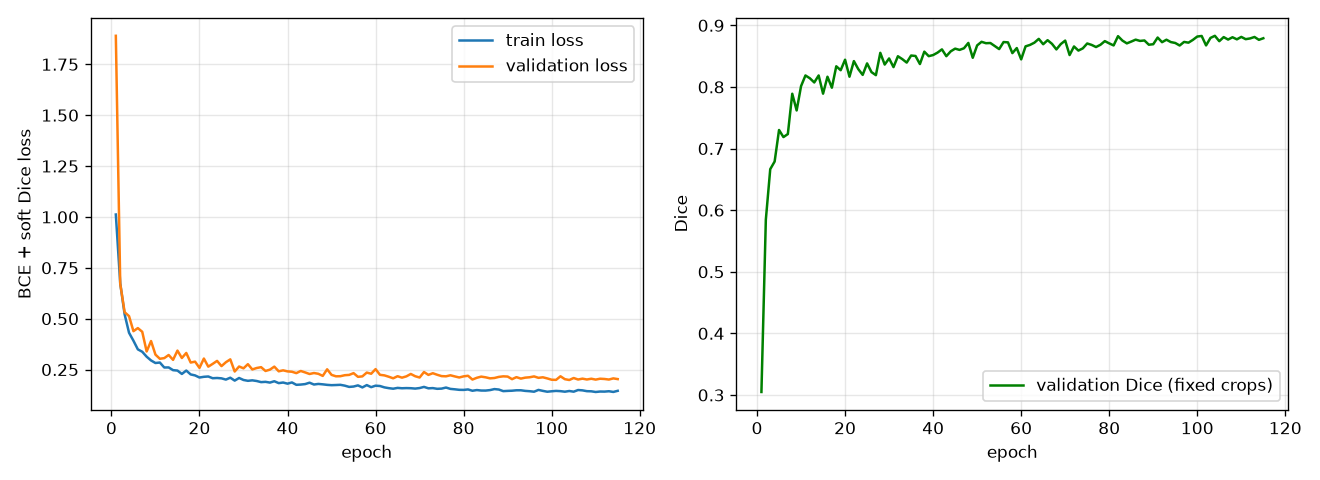
\includegraphics[width=0.92\textwidth]{figures/curves_final.png}
\caption{Final model (E2): training and validation loss (left) and validation Dice (right) per epoch. The validation loss does not climb back up: no clear overfitting.}
\label{fig:curves}
\end{figure}

\subsection{Final test on FIVES}
\begin{table}[h]
\centering\small
\begin{tabular}{@{}lccccc@{}}
\toprule
\textbf{Metric} & \textbf{All (200)} & \textbf{AMD} & \textbf{Diab. retino.} & \textbf{Glaucoma} & \textbf{Healthy} \\
\midrule
Dice & \textbf{0.889} (0.873 -- 0.903) & 0.917 & 0.888 & 0.850 & 0.902 \\
clDice & 0.897 (0.881 -- 0.911) & 0.921 & 0.895 & 0.851 & 0.921 \\
Precision & 0.919 & 0.934 & 0.935 & 0.916 & 0.891 \\
Recall & 0.874 & 0.906 & 0.854 & 0.820 & 0.917 \\
\bottomrule
\end{tabular}
\caption{FIVES test of the final model. IoU 0.813; specificity 0.994; median Dice 0.914; thin-vessel recall 0.458. Gain over version 1: +0.015 (0.012 -- 0.017).}
\end{table}

\begin{figure}[h]
\centering
\includegraphics[width=\textwidth]{figures/private/example_67D.png}\\[2pt]
\includegraphics[width=\textwidth]{figures/private/example_4A.png}
\caption{Two FIVES test images: photograph, expert mask, prediction, overlay (prediction in green). FIVES images, Jin et al.\ 2022, CC BY 4.0 licence.}
\end{figure}

\textbf{Pre-trained reference.} A U-Net with a ResNet34 encoder \cite{resnet} pre-trained on ImageNet (24.4 million parameters, same data and same budget) reaches a Dice of \textbf{0.907} (0.891 -- 0.921). It is better on every metric, which is expected: it starts with filters learned on 1.2 million images and is three times larger. Our model is a sound, fully explainable baseline, not the best possible model.

\subsection{External test on CHASE\_DB1 and comparison with a human}
\begin{table}[h]
\centering\small
\begin{tabular}{@{}lcccc@{}}
\toprule
\textbf{Comparison (against observer 1)} & \textbf{Dice} & \textbf{clDice} & \textbf{Sensitivity} & \textbf{Specificity} \\
\midrule
Our final model & 0.766 & 0.835 & 0.908 & 0.949 \\
Pre-trained model & 0.770 & 0.840 & 0.914 & 0.949 \\
\textbf{Observer 2 (human)} & \textbf{0.777} & 0.835 & 0.769 & 0.978 \\
\bottomrule
\end{tabular}
\caption{CHASE\_DB1, 28 images of 14 children, never used for training or for any choice. CHASE images are enlarged by a factor of $\approx1.31$ to match the pixels per degree of FIVES.}
\end{table}
\begin{itemize}
  \item The Dice drops from 0.889 (FIVES) to 0.766 (CHASE); even two experts only agree at 0.777 on this dataset.
  \item The model makes a different kind of error than the human: much higher sensitivity (+0.139, interval 0.103 -- 0.176) and lower precision (0.66 vs 0.80). It marks \textbf{more} pixels than the experts.
  \item The gains of version 2 and the advantage of the pre-trained model vanish on CHASE: the limit comes from the change of camera and population, not from model size.
\end{itemize}

\subsection{The worst images}
The three worst images were inspected by eye. For \texttt{train/174\_D} (validation, Dice 0.15), the expert mask \textbf{does not match the photograph}: an annotation error in the dataset (figure~\ref{fig:worst}). The two worst test images (\texttt{122\_G}, \texttt{123\_G}) are very dark, blurry photographs where the expert traced only a few segments.

\begin{figure}[h]
\centering
\includegraphics[width=0.75\textwidth]{figures/private/worst_174D.png}
\caption{\texttt{train/174\_D}: photograph, expert mask, prediction. The vessel tree in the expert mask does not match the one in the photograph; the prediction follows the visible vessels.}
\label{fig:worst}
\end{figure}

% ---------------------------------------------------------------------------
\section{From mask to measurement: MedSkel}

\subsection{Centre lines}
To measure the length of a vessel or count its branch points, we need its centre line (skeleton). Two methods are compared:
\begin{itemize}
  \item \textbf{Thinning} (standard method, \texttt{scikit-image}): remove border pixels, layer by layer, until a 1-pixel line remains. Simple, but sensitive to small bumps on the outline, which become small fake branches.
  \item \textbf{MedSkel} \cite{saidou}: the outline is approximated by a polygon (simplification with $\varepsilon=4$ px), then the centre line is made of the points at equal distance from both borders, computed with a Voronoi diagram. The code of the original \texttt{medskel} project is imported read-only.
\end{itemize}

\textbf{Measurements} (in pixels; no validated conversion to millimetres): vessel density (share of the retinal field covered), fractal dimension (box counting: slope of $\log N(s)$ against $\log(1/s)$), total length, number of branch points, median width, median tortuosity. Tortuosity depends too much on the method (about 1.07 with thinning because of the staircase effect, 1.01 with MedSkel because of the simplification): it is not interpreted.

\textbf{A bias fixed.} In the original MedSkel code, a branch's width is computed only at the vertices kept after simplification, mostly at the ends, where the vessel narrows: a 12-pixel-wide test vessel is measured as 1.3 pixels. Without changing the original repository, width is measured here the same way for both methods (distance transform along the centre line). The \emph{length} results of the original project are not affected.

\textbf{Check.} Between the two CHASE observers, total length changes by 9.3\pct\ (thinning) and 3.2\pct\ (MedSkel): exactly the values of the original project, which confirms the two codes are connected correctly.

\subsection{Stability of the measurements}
The relative difference between two measurements $a$ and $b$ is $|a-b|/\frac{a+b}{2}$.
\begin{table}[h]
\centering\small
\begin{tabular}{@{}lcc|cc@{}}
\toprule
 & \multicolumn{2}{c|}{\textbf{FIVES test: CNN vs expert}} & \multicolumn{2}{c}{\textbf{CHASE: human 2 vs human 1}} \\
\textbf{Measure} & Thinning & MedSkel & Thinning & MedSkel \\
\midrule
Vessel density & 0.057 & (same mask) & 0.127 & (same mask) \\
Total length & 0.068 & 0.063 & 0.093 & 0.032 \\
Branch points & 0.532 & \textbf{0.258} & 0.216 & 0.122 \\
Median width & 0.178 & \textbf{0.133} & 0.175 & 0.173 \\
\bottomrule
\end{tabular}
\caption{Median relative difference (lower = more stable). FIVES: 200 images, Wilcoxon test $p<0.001$ for all four skeleton measures.}
\end{table}

On FIVES, replacing the expert mask with the network mask changes density and length by about 6 to 7\pct. With MedSkel, the number of branch points changes \textbf{half as much} as with thinning. On CHASE, however, the network's measurements are further from the experts than the experts are from each other (density: 0.302 vs 0.127; width: 0.39 to 0.67 vs 0.17), a direct consequence of the over-marking seen in the previous section (figure~\ref{fig:chase}).

\begin{figure}[h]
\centering
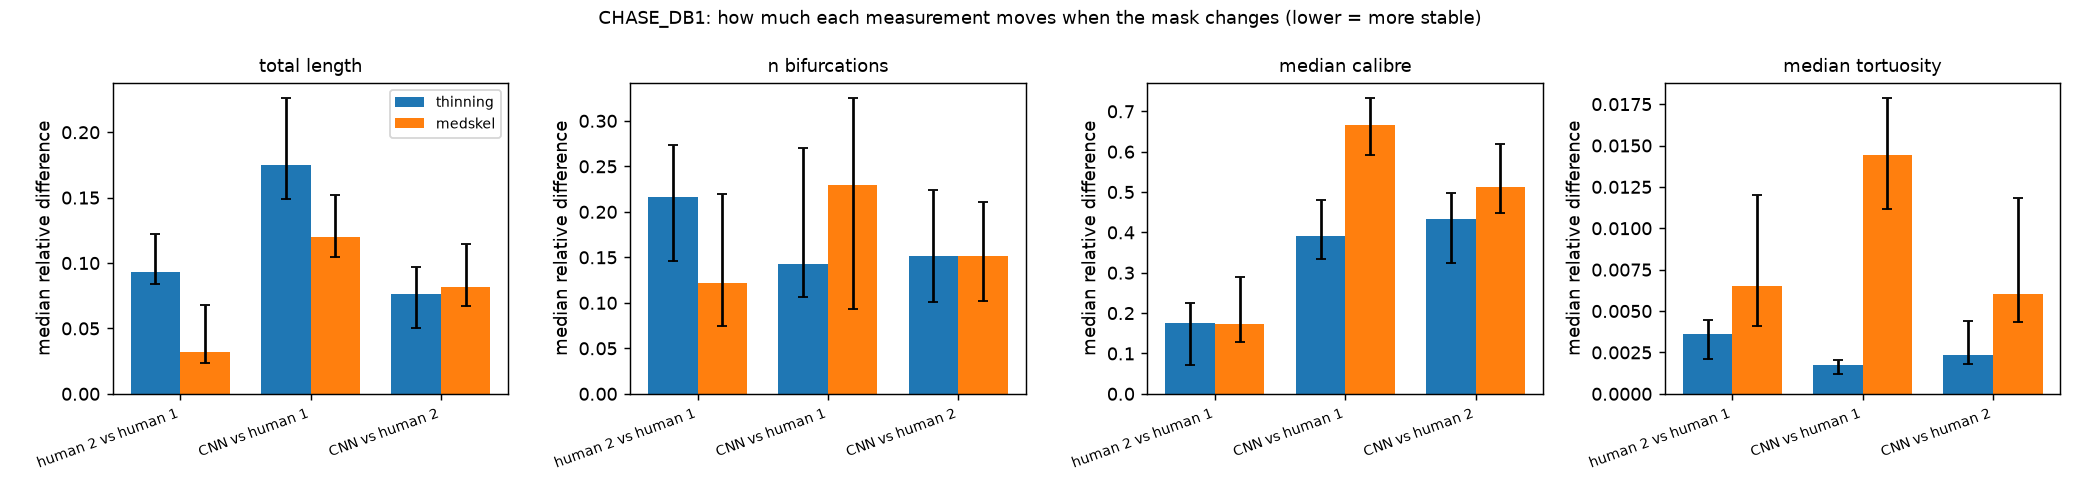
\includegraphics[width=\textwidth]{figures/chase_agreement.png}
\caption{CHASE\_DB1: median relative difference of each measure between human 2 and human 1, and between the network and each human, for both skeleton methods.}
\label{fig:chase}
\end{figure}

\subsection{Measurements and disease groups}
\begin{table}[h]
\centering\small
\begin{tabular}{@{}lcccc@{}}
\toprule
\textbf{Measure (median)} & \textbf{Healthy (200)} & \textbf{AMD (194)} & \textbf{Diab. retino. (199)} & \textbf{Glaucoma (198)} \\
\midrule
Vessel density & 11.6\pct & 10.0\pct & 9.6\pct & 9.4\pct \\
Fractal dimension & 1.528 & 1.501 & 1.497 & 1.490 \\
Total length (px) & 30{,}435 & 26{,}620 & 23{,}732 & 25{,}159 \\
Branch points & 177 & 138 & 142 & 155 \\
\bottomrule
\end{tabular}
\caption{FIVES expert masks (training + test, duplicates counted once, faulty masks excluded), thinning. Kruskal--Wallis $p<0.001$ for each measure; each disease vs healthy: Holm-corrected Mann--Whitney, $p<0.001$.}
\end{table}

All three disease groups show lower vessel density, fractal dimension, total length and number of branch points than healthy eyes. The same pattern appears with the network masks on the 200 test images (figure~\ref{fig:groups}).

\begin{figure}[h]
\centering
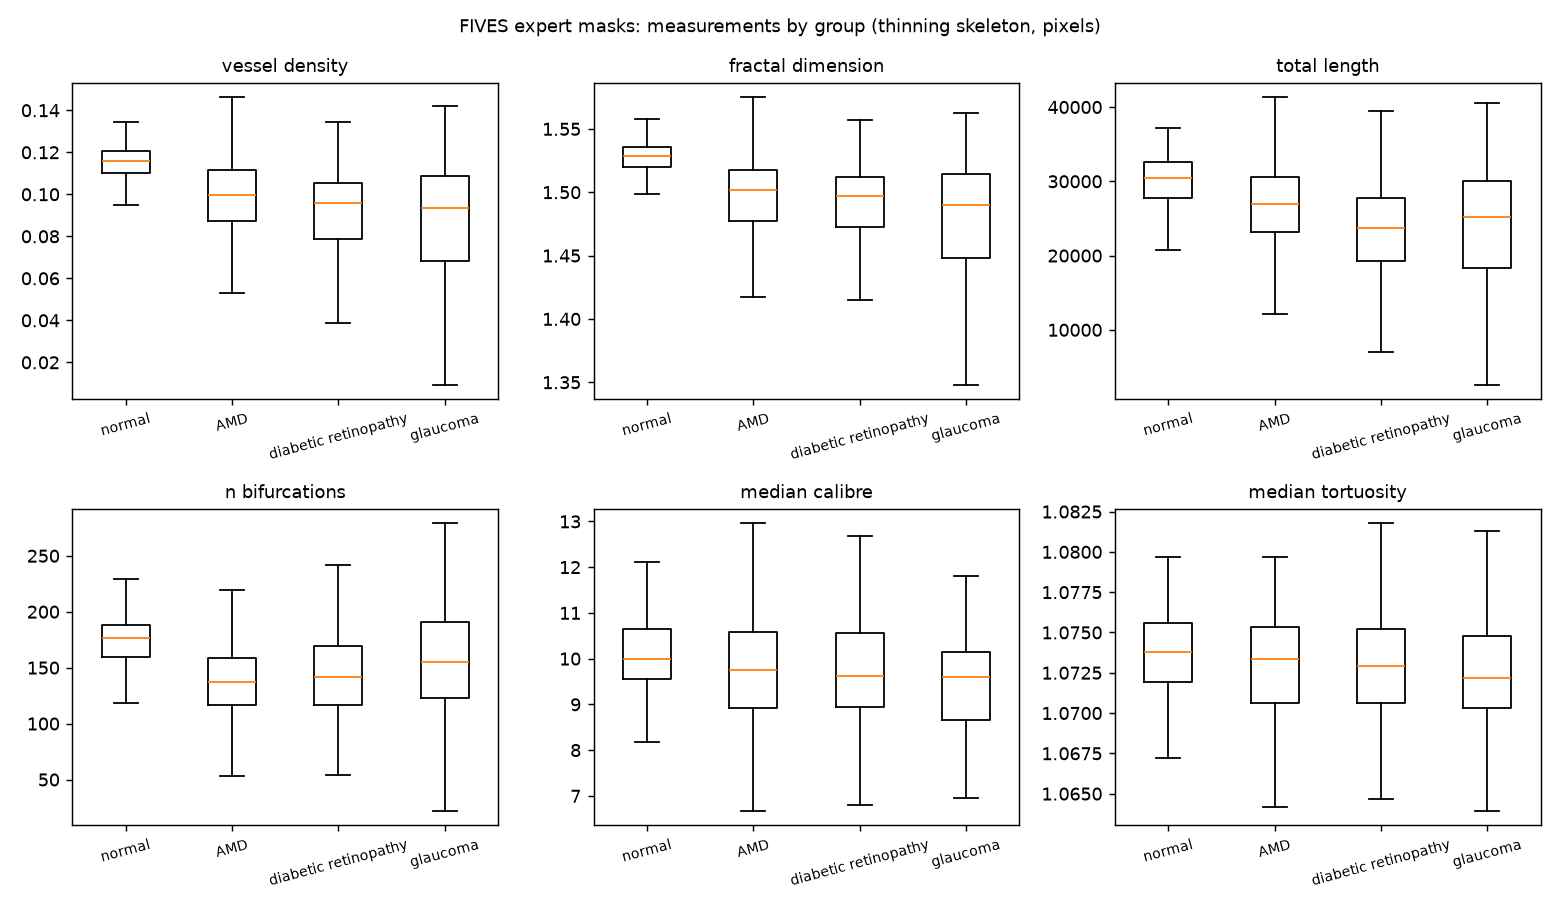
\includegraphics[width=0.95\textwidth]{figures/groups_expert.png}
\caption{Distribution of the measurements per group (FIVES expert masks, thinning, pixels).}
\label{fig:groups}
\end{figure}

\textbf{Classify one eye from the measurements?} A logistic regression on the 6 measurements, trained on the training images and evaluated once on the 200 test images:
\begin{center}\small
\begin{tabular}{@{}llcc@{}}
\toprule
\textbf{Centre lines} & \textbf{Test masks} & \textbf{Balanced accuracy (chance: 0.25)} & \textbf{AUC healthy vs DR} \\
\midrule
Thinning & expert & 0.488 & 0.818 \\
Thinning & network & 0.449 & 0.842 \\
MedSkel & expert & 0.457 & 0.748 \\
MedSkel & network & 0.453 & 0.805 \\
\bottomrule
\end{tabular}
\end{center}
With shuffled labels, the mean accuracy is 0.251 ($p\le0.004$): the measurements carry real information, and the full chain photo $\to$ network $\to$ measurements works almost as well as with expert masks. But the classifier is wrong more than half the time. As in the literature \cite{yusufu}, the link is clear \textbf{at the group level} and too weak \textbf{for one person}. These are associations in a single dataset, which may also reflect image quality, lesions hiding vessels, or how experts annotate diseased eyes.

% ---------------------------------------------------------------------------
\section{Application}
A local application (Gradio) runs every step: loading a photograph, segmentation (before/after slider), MedSkel centre lines, a table of measurements and a chart placing the eye among the 4 groups (figure~\ref{fig:app}). Each measurement is compared with 50 healthy FIVES test eyes processed exactly the same way (network then MedSkel). The measurements can be exported as CSV. The application clearly states that it is not a diagnosis, and on purpose offers no individual disease prediction. It starts with a double click (\texttt{MedSkel AI.bat}); a full analysis takes about 6 seconds on the laptop GPU.

\begin{figure}[h]
\centering
\begin{minipage}{0.47\textwidth}\centering\includegraphics[width=\textwidth]{figures/private/app_top.png}\end{minipage}\hfill
\begin{minipage}{0.5\textwidth}\centering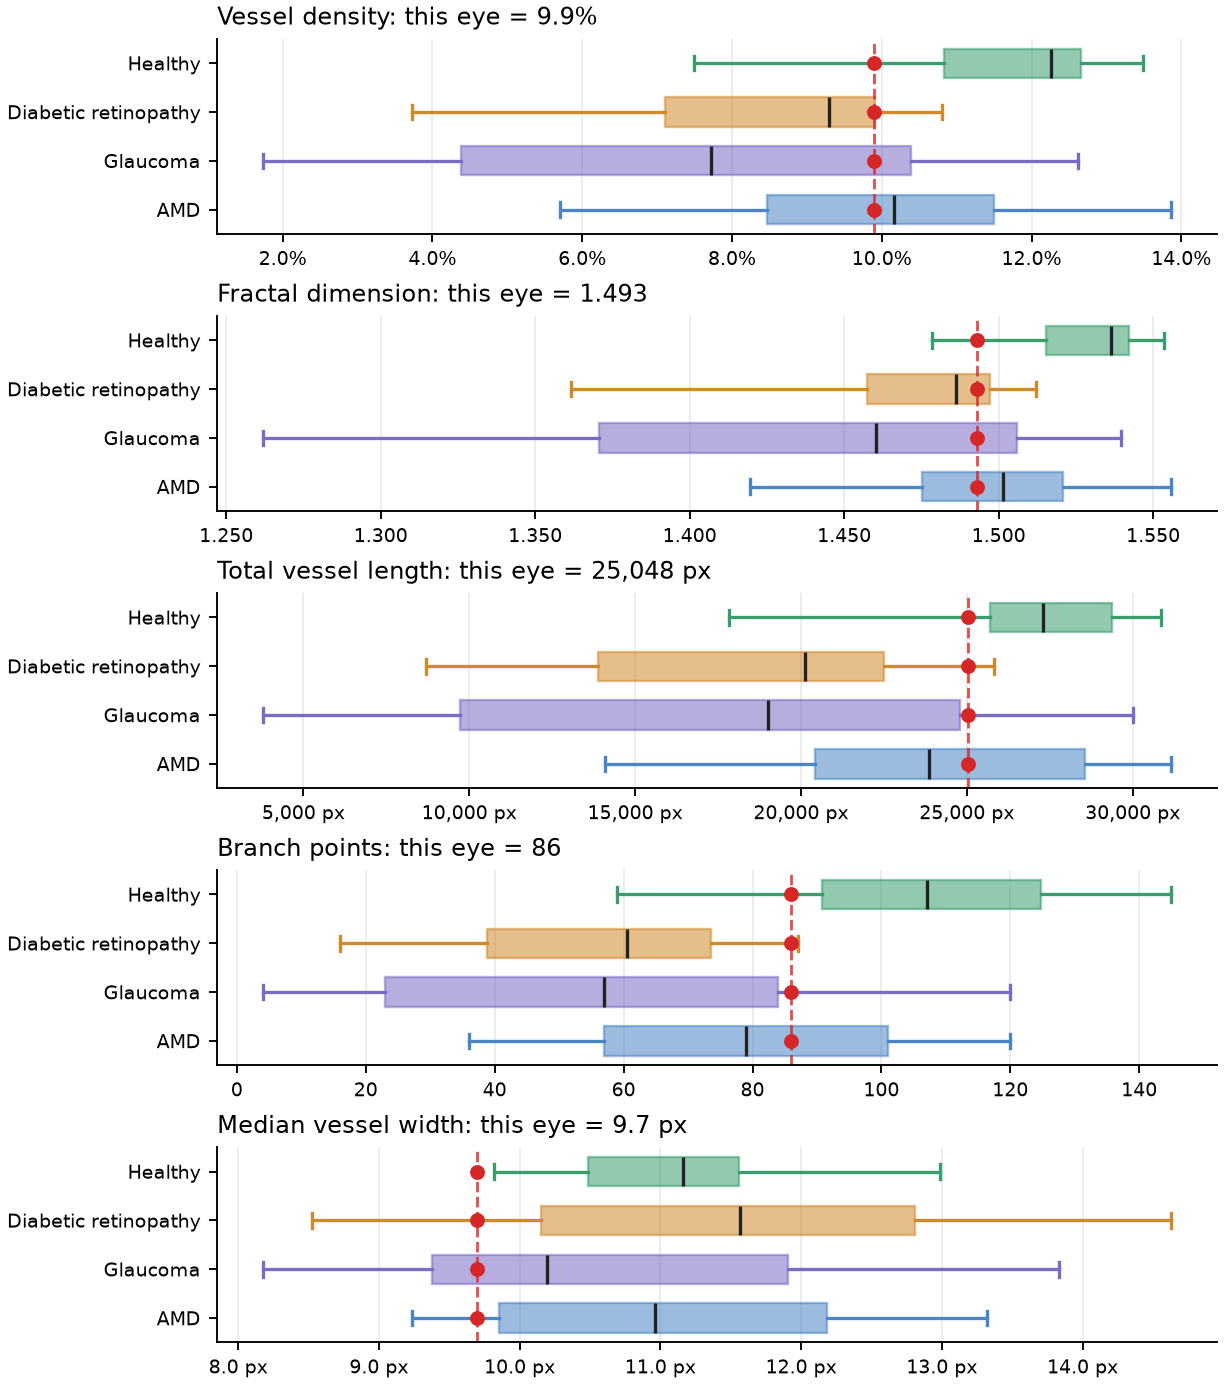
\includegraphics[width=\textwidth]{figures/eye_chart.png}\end{minipage}
\caption{Left: the application (vessels in green, MedSkel centre lines in red). Right: position of a test eye (red dot) among the 4 FIVES groups; the distributions overlap a lot.}
\label{fig:app}
\end{figure}

% ---------------------------------------------------------------------------
\section{Discussion and limitations}
\begin{itemize}
  \item \textbf{Thin vessels}: only about 46\pct\ of the pixels of vessels 1 to 4 pixels wide are found; neither longer training nor the clDice loss solved this.
  \item \textbf{Generalisation}: on another camera (CHASE), the Dice drops and the network over-marks; the measurements do not transfer yet.
  \item \textbf{Units}: measurements in pixels only.
  \item \textbf{Patients}: patient independence between training and test is not guaranteed in FIVES.
  \item \textbf{Variability}: a single training run per setting (one seed); very small differences should not be over-read.
  \item \textbf{Test reused}: the FIVES test was evaluated twice (version 1 and final version), always after the choices were frozen.
  \item \textbf{Clinical use}: none. This is not a medical device.
\end{itemize}

% ---------------------------------------------------------------------------
\section{Conclusion and future work}
A 7.8-million-parameter U-Net, trained from scratch on a laptop GPU, segments FIVES retinal vessels with a Dice of 0.889 and, on an external dataset, reaches an agreement close to that between two experts. Connected to the geometric method MedSkel, it gives more stable measurements than classical thinning, and these measurements reproduce known differences between healthy and diseased eyes, without allowing an individual diagnosis.

Future work: improve thin vessels (width-weighted loss, finer resolution), adapt the model to other cameras (domain augmentation, extra data), calibrate a millimetre scale, repeat training with several seeds, and, in the longer term, validate the measurements on clinical data with an ophthalmology department.

% ---------------------------------------------------------------------------
\appendix
\section{Code and reproduction}
The code is in Python/PyTorch: \url{https://github.com/MouhssineElBoumshouli/medskel-ai}. Data and weights are not in Git.
\begin{center}\small
\begin{tabularx}{\textwidth}{@{}lX@{}}
\toprule
\textbf{File} & \textbf{Role} \\
\midrule
\texttt{src/medskel\_ai/data.py} & FIVES audit, image/mask pairing, split, tiles \\
\texttt{src/medskel\_ai/model.py} & the U-Net \\
\texttt{src/medskel\_ai/train.py} & training (BCE + Dice, Adam, mixed precision) \\
\texttt{src/medskel\_ai/predict.py} & tiled prediction, test-time flips \\
\texttt{src/medskel\_ai/evaluate.py} & metrics, threshold choice, bootstrap \\
\texttt{src/medskel\_ai/chase.py} & CHASE\_DB1 external test \\
\texttt{src/medskel\_ai/morphometry.py} & centre lines and measurements \\
\texttt{src/medskel\_ai/study.py} & measurement study (stability, groups, classifier) \\
\texttt{app.py}, \texttt{MedSkel AI.bat} & application \\
\texttt{tests/} & automatic tests (pytest) on synthetic data \\
\bottomrule
\end{tabularx}
\end{center}
\begin{verbatim}
python -m medskel_ai.train --minutes 150          # training
python -m medskel_ai.evaluate --split val         # threshold choice
python -m medskel_ai.evaluate --split test        # final test (once)
python -m medskel_ai.study all                    # measurement study
python app.py                                     # application
\end{verbatim}

% ---------------------------------------------------------------------------
\begin{thebibliography}{99}\small
\bibitem{unet} O. Ronneberger, P. Fischer, T. Brox. \emph{U-Net: Convolutional Networks for Biomedical Image Segmentation}. MICCAI, 2015.
\bibitem{fives} K. Jin et al. \emph{FIVES: A Fundus Image Dataset for Artificial Intelligence based Vessel Segmentation}. Scientific Data 9, 475, 2022. doi:10.1038/s41597-022-01564-3.
\bibitem{chase} M. M. Fraz et al. \emph{An Ensemble Classification-Based Approach Applied to Retinal Blood Vessel Segmentation}. IEEE Trans. Biomedical Engineering 59, 2012.
\bibitem{saidou} N. Saidou et al. \emph{A Novel Method of Skeletonization of Complex Shapes Based on Bisectors}. 2024. doi:10.1142/S2972370123500083.
\bibitem{cldice} S. Shit et al. \emph{clDice -- a Novel Topology-Preserving Loss Function for Tubular Structure Segmentation}. CVPR, 2021.
\bibitem{vnet} F. Milletari, N. Navab, S.-A. Ahmadi. \emph{V-Net: Fully Convolutional Neural Networks for Volumetric Medical Image Segmentation}. 3DV, 2016.
\bibitem{adam} D. P. Kingma, J. Ba. \emph{Adam: A Method for Stochastic Optimization}. ICLR, 2015.
\bibitem{bn} S. Ioffe, C. Szegedy. \emph{Batch Normalization: Accelerating Deep Network Training by Reducing Internal Covariate Shift}. ICML, 2015.
\bibitem{resnet} K. He, X. Zhang, S. Ren, J. Sun. \emph{Deep Residual Learning for Image Recognition}. CVPR, 2016.
\bibitem{yusufu} M. Yusufu et al. \emph{Population-Based Normative Reference for Retinal Microvascular Atlas}. Ophthalmology Science, 2025. doi:10.1016/j.xops.2025.100723.
\end{thebibliography}

\end{document}
